% The contents of this file is 
% Copyright (c) 2009-  Charles R. Severance, All Righs Reserved

\chapter{Utilizando Web Services}
%\chapter{Using Web Services}

Uma vez que se tornou mais fácil retornar e analisar documentos
sob HTTP utilizando programas, não levará muito tempo para desenvolvermos
um sistema onde começamos a produzir documentos que serão
especificamente projetados para serem utilizados por outros
programas (i.e., não é o HTML que é mostrado no navegador).
%Once it became easy to retrieve documents and parse documents 
%over HTTP using programs, it did not take long to develop 
%an approach where we started producing documents that were specifically
%designed to be consumed by other 
%programs (i.e., not HTML to be displayed in a browser).

Existem dois formatos comuns que usamos para trocar dados através da web.
O ``eXtensible Markup Language'' ou XML têm sido utilizado por muito tempo
e se adequa melhor na troca de dados do tipo document-style. Quando programas somente
querem trocar dicionários, listas, ou outra informação interna entre eles, 
costumam utilizar o JavaScript Object Notation ou JSON (sobre \url{www.json.org}).
Iremos estudar ambos os formatos.
%There are two common formats that we use when exchanging data across the web.
%The ``eXtensible Markup Language'' or XML has been in use for a very long time 
%and is best suited for exchanging document-style data.   When programs just want 
%to exchange dictionaries, lists, or other internal information with each other,
%they use JavaScript Object Notation or JSON (see \url{www.json.org}).  
%We will look at both formats.

\section{eXtensible Markup Language - XML}
%\section{eXtensible Markup Language - XML}

O XML é bem parecido com o HTML, porém o XML é mais estruturado
que o HTML. Aqui está um exemplo de um documento XML:
%XML looks very similar to HTML, but XML is more structured 
%than HTML.  Here is a sample of an XML document:

\beforeverb
\begin{verbatim}
<person>
  <name>Chuck</name>
  <phone type="intl">
     +1 734 303 4456
   </phone>
   <email hide="yes"/>
</person>
\end{verbatim}
\afterverb

É mais fácil pensar em um documento XML como uma estrutura em árvore
onde tem uma tag no topo {\tt person} e outras tags como {\tt phone}
são escritas como \emph{filhos} dos nós pai.
%Often it is helpful to think of an XML document as a tree structure
%where there is a top tag {\tt person} and other tags such as {\tt phone}
%are drawn as \emph{children} of their parent nodes.

\beforefig
\centerline{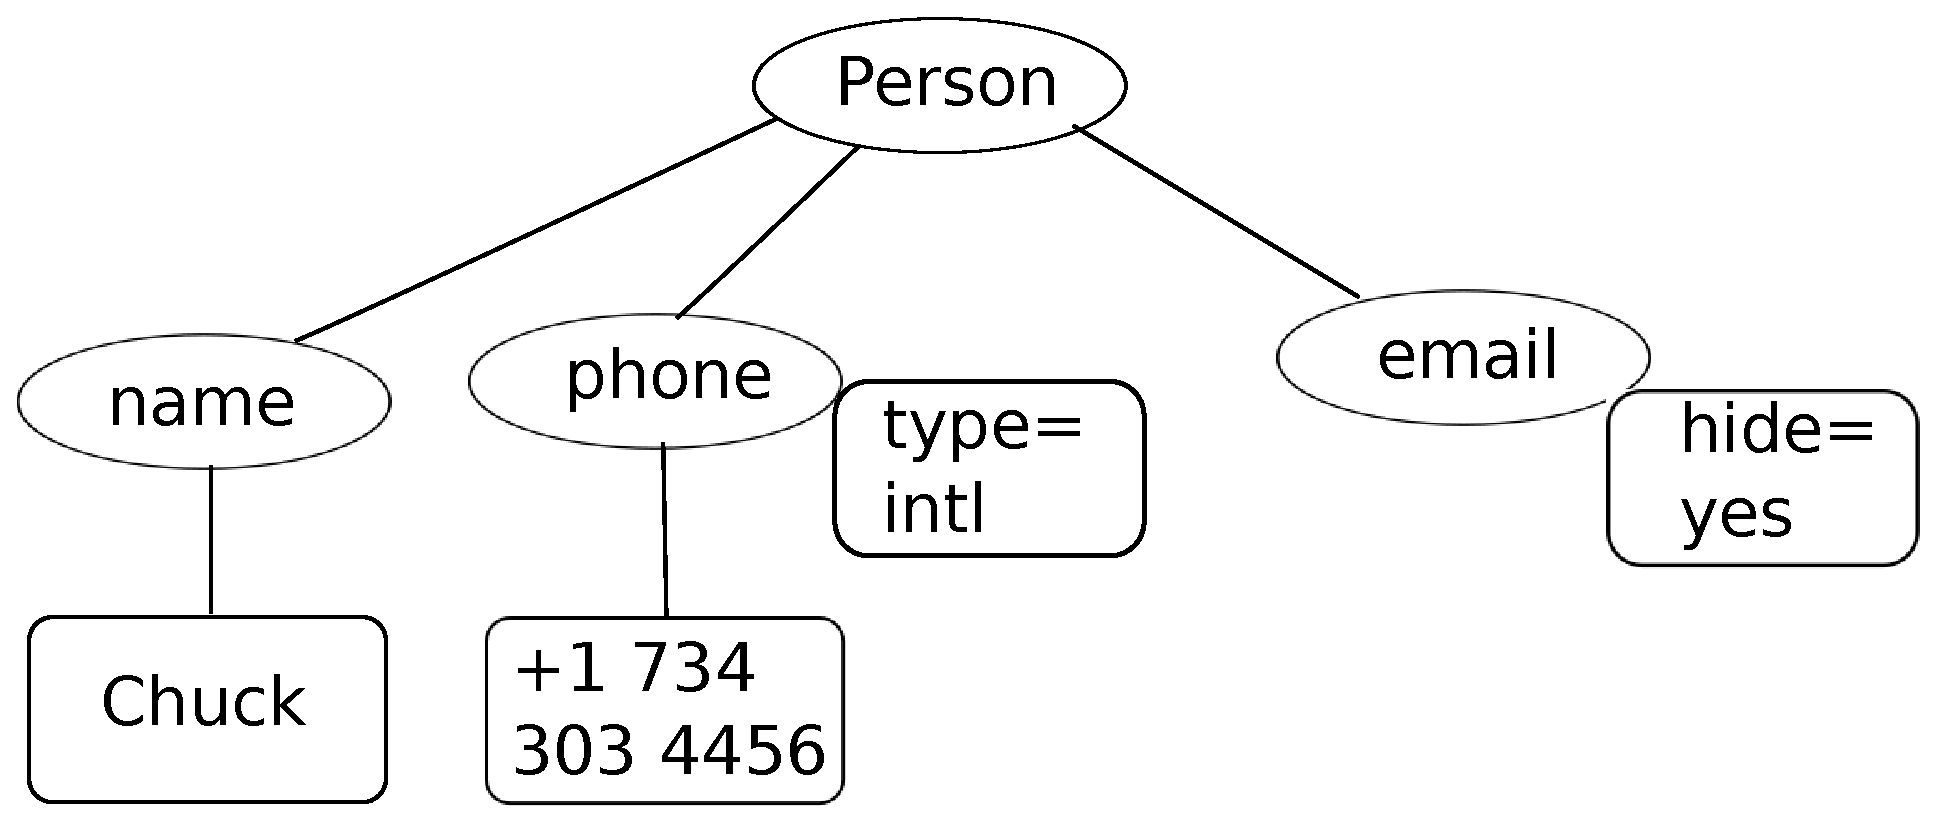
\includegraphics[height=1.50in]{figs2/xml-tree.eps}}
\afterfig

\section{Analisando o XML}
%\section{Parsing XML}

\index{ElementTree}
\index{ElementTree!fromstring}
\index{ElementTree!find}

Aqui está uma simples aplicação que analisa um XML
e extrai alguns elementos do XML:
%Here is a simple application that parses some XML
%and extracts some data elements from the XML:

\beforeverb
\begin{verbatim}
import xml.etree.ElementTree as ET

data = '''
<person>
  <name>Chuck</name>
  <phone type="intl">
     +1 734 303 4456
   </phone>
   <email hide="yes"/>
</person>'''

tree = ET.fromstring(data)
print 'Name:',tree.find('name').text
print 'Attr:',tree.find('email').get('hide')
\end{verbatim}
\afterverb

Ao chamar {\tt fromstring} é feita a conversão da string que 
representa o XML em uma ``árvore'' de nós XML. Quando o
XML está em uma árvore, nós temos uma série de métodos que
podemos chamar para extrair informações do XML.
%Calling {\tt fromstring} converts the string representation
%of the XML into a ``tree'' of XML nodes.  When the
%XML is in a tree, we have a series of methods we can call to 
%extract portions of data from the XML.  

A função {\tt find} varre a árvore do XML
e retorna um {\bf nó} que corresponde a essa tag específica.
Cada nó pode conter algum texto, alguns atributos (como hide), e
algum nó ``filho''. Cada nó pode ser o início de uma árvore de nós.
%The {\tt find} function searches through the 
%XML tree and retrieves a {\bf node} that matches the specified tag.
%Each node can have some text, some attributes (like hide), and
%some ``child'' nodes.   Each node can be the top of a tree of nodes.

\beforeverb
\begin{verbatim}
Name: Chuck
Attr: yes
\end{verbatim}
\afterverb

Ao utilizar um analisador de XML como o {\tt ElementTree} tem-se a
vantagem que, como o XML deste exemplo é bastante simples, 
se tem muitas regras em relação à validação do XML e usar o 
{\tt ElementTree} nos permitirá extrair informações do XML sem
nos preocuparmos com as regras de sintaxe do XML.
%Using an XML parser such as {\tt ElementTree} has the advantage
%that while the XML in this example is quite simple, it turns
%out there are many rules regarding valid XML and using 
%{\tt ElementTree} allows us to extract data from XML without 
%worrying about the rules of XML syntax.

\section{Percorrendo os nós}
%\section{Looping through nodes}

\index{ElementTree!findall}
\index{ElementTree!get}
Frequentemente um XML tem múltiplos nós e precisamos escrever
um laço para processar todos os nós. No programa a seguir,
nós percorremos todos os nós do {\tt user}:
%Often the XML has multiple nodes and we need to write a loop
%to process all of the nodes.  In the following program, 
%we loop through all of the {\tt user} nodes:

\beforeverb
\begin{verbatim}
import xml.etree.ElementTree as ET

input = '''
<stuff>
    <users>
        <user x="2">
            <id>001</id>
            <name>Chuck</name>
        </user>
        <user x="7">
            <id>009</id>
            <name>Brent</name>
        </user>
    </users>
</stuff>'''

stuff = ET.fromstring(input)
lst = stuff.findall('users/user')
print 'User count:', len(lst)

for item in lst:
    print 'Name', item.find('name').text
    print 'Id', item.find('id').text
    print 'Attribute', item.get('x')
\end{verbatim}
\afterverb

O método {\tt findall} retorna uma lista do Python com subárvores
que representam a estrutura {\tt user} da árvore do XML. Então nós 
podemos escrever um laço {\tt for} que procura em cada nó user,
e imprime os elementos {\tt name} e {\tt id} assim como o 
atributo {\tt x} do nó {\tt user}.
%The {\tt findall} method retrieves a Python list of subtrees that
%represent the {\tt user} structures in the XML tree.  Then we can 
%write a {\tt for} loop that looks at each of the user nodes, and 
%prints the {\tt name} and {\tt id} text elements as well as the 
%{\tt x} attribute from the {\tt user} node.

\beforeverb
\begin{verbatim}
User count: 2
Name Chuck
Id 001
Attribute 2
Name Brent
Id 009
Attribute 7
\end{verbatim}
\afterverb

\section{JavaScript Object Notation - JSON}
%\section{JavaScript Object Notation - JSON}
\index{JSON}
\index{JavaScript Object Notation}

O formato JSON foi inspirado no formato do objeto array utilizado na linguagem JavaScript.
Mas como o Python foi inventado antes do JavaScript, a sintaxe que o Python utiliza
para dicionários e listas influenciaram na sintaxe do JSON. Então o formato JSON é
bem parecido com a combinação de listas e dicionários do Python.
%The JSON format was inspired by the object and array format used in the JavaScript
%language.  But since Python was invented before JavaScript, Python's syntax
%for dictionaries and lists influenced the syntax of JSON.  So the format of JSON
%is nearly identical to a combination of Python lists and dictionaries.

Aqui está uma codificação JSON que é quase equivalente ao simples XML mostrado antes:
%Here is a JSON encoding that is roughly equivalent to the simple XML from above:

\beforeverb
\begin{verbatim}
{
  "name" : "Chuck",
  "phone" : {
    "type" : "intl",
    "number" : "+1 734 303 4456"
   },
   "email" : {
     "hide" : "yes"
   }
}
\end{verbatim}
\afterverb

Você pode notar algumas diferenças. Primeira, no XML, nós podemos adicionar
atributos como ``intl'' à tag ``phone''. No JSON, nós simplesmente temos chaves de
valores pares. Além de que a tag ``person'' não existe mais, pois foi substituída por
um conjunto de chaves externas.
%You will notice some differences.  First, in XML, we can add attributes like
%``intl'' to the ``phone'' tag.  In JSON, we simply have key-value pairs.  Also
%the XML ``person'' tag is gone, replaced by a set of outer curly braces.  

No geral, a estrutura JSON é mais simples que a do XML por conta do JSON ter menos
capacidades que o XML. Mas o JSON tem a vantagem de mapear {\em diretamente} para alguma
combinação de dicionários e listas. Como quase todas as linguagens de programação 
tem algo equivalente aos dicionários e listas do Python, o JSON é um formato natural 
para fazer dois programas cooperarem e trocarem dados.
%In general, JSON structures are simpler than XML because JSON has fewer capabilities
%than XML.  But JSON has the advantage that it maps {\em directly} to some combination
%of dictionaries and lists.   And since nearly all programming languages 
%have something equivalent to Python's dictionaries and lists, JSON is a very
%natural format to have two cooperating programs exchange data.

JSON está facilmente se tornando o formato escolhido para realizar troca de dados
entre aplicações por conta de sua simplicidade se comparado ao XML.
%JSON is quickly becoming the format of choice for nearly all data exchange between 
%applications because of its relative simplicity compared to XML.

\section{Analisando o JSON}
%\section{Parsing JSON}

Nós podemos construir nosso JSON utilizando dicionários (objetos) e listas conforme
necessário. Neste exemplo, vamos representar uma lista de usuários onde cada
usuário é um conjunto de pares de valor-chave (i.e., um dicionário). Então nós temos
uma lista de dicionários.
%We construct our JSON by nesting dictionaries (objects) and lists as needed.  In 
%this example, we represent a list of users where each user is a set of 
%key-value pairs (i.e., a dictionary).  So we have a list of dictionaries.

No programa a seguir, nós usamos a biblioteca padrão {\bf json} para analisar
o JSON e ler as informações. Compare ele de perto com a informação equivalente em XML
abaixo. O JSON tem menos detalhes, então nós devemos previamente saber que
estamos pegando uma lista e essa lista é composta por usuários, e cada usuário é um valor de 
chave. O JSON é mais sucinto (uma vantagem) mas também é menos auto explicativo 
(uma desvantagem).
%In the following program, we use the built-in {\bf json} library to parse 
%the JSON and read through the data.   Compare this closely to the equivalent
%XML data and code above.  The JSON has less detail, so we must know in advance 
%that we are getting a list and that the list is of users and each user is a
%set of key-value pairs.  The JSON is more succinct (an advantage) but also is 
%less self-describing (a disadvantage).

\beforeverb
\begin{verbatim}
import json

input = '''
[
  { "id" : "001",
    "x" : "2",
    "name" : "Chuck"
  } ,
  { "id" : "009",
    "x" : "7",
    "name" : "Brent"
  } 
]'''

info = json.loads(input)
print 'User count:', len(info)

for item in info:
    print 'Name', item['name']
    print 'Id', item['id']
    print 'Attribute', item['x']
\end{verbatim}
\afterverb
%

Se você comparar o código para extrair as informações do JSON e XML analisados,
você verá que o que nós pegamos do {\bf json.loads()} é uma lista Python
que nós percorremos com um {\tt for} loop, e cada item dentro desta lista
é um dicionario Python. Uma vez que o JSON foi analisado, nós pudemos usar o
operador de índice do Python para extrair varias informações de cada usuário.
Nós não precisamos usar a biblioteca JSON para percorrer o JSON analisado, 
pois ela retornará uma informação que já é uma estrutura do próprio Python.
%If you compare the code to extract data from the parsed JSON and XML
%you will see that what we get from {\bf json.loads()} is a Python list
%which we traverse with a {\tt for} loop, and each item within that list
%is a Python dictionary.  Once the JSON has been parsed, we can use the Python
%index operator to extract the various bits of data for each user.  We don't
%have to use the JSON library to dig through the parsed JSON, since the returned
%data is simply native Python structures.

A saída deste programa é exatamente a mesma que a versão em XML abaixo.
%The output of this program is exactly the same as the XML version above.

\beforeverb
\begin{verbatim}
User count: 2
Name Chuck
Id 001
Attribute 2
Name Brent
Id 009
Attribute 7
\end{verbatim}
\afterverb

Em geral, existe uma tendência da indústria utilizar cada vez mais o JSON
do que o XML em serviços web. Por conta do JSON ser mais simples e mais
direcionado para estruturas nativas que já existem nas linguagens de
programação, a análise e extração de dados é usualmente simples e mais direta
utilizando JSON. Mas o XML é mais auto explicativo que o JSON então terá
algumas aplicações em que o XML detém a vantagem. Por exemplo, a maioria de 
processadores de palavras armazenam documentos internamente utilizando XML
em vez de JSON.
%In general, there is an industry trend away from XML and towards JSON for 
%web services.  Because the JSON is simpler and more directly maps to native 
%data structures we already have in programming languages, the parsing 
%and data extraction code is usually simpler and more direct when using JSON.
%But XML is more self-descriptive than JSON and so there are 
%some applications where XML retains an advantage.  For example, most word 
%processors store documents internally using XML rather than JSON.

\section{Interfaces de Programação de Aplicação}
%\section{Application Programming Interfaces}

Nós agora temos a habilidade de trocar dados entre aplicações utilizando 
HyperText Transport Protocol (HTTP) e uma forma de representar dados complexos
que nós estamos enviando e recebendo entre estas aplicações utilizando 
eXtensible Markup Language (XML) ou JavaScript Object Notation (JSON).
%We now have the ability to exchange data between applications using HyperText
%Transport Protocol (HTTP) and a way to represent complex data that we are 
%sending back and forth between these applications using eXtensible 
%Markup Language (XML) or JavaScript Object Notation (JSON).

O próximo passo é começar a definir e documentar ``contratos'' entre
aplicações utilizando essas técnicas. O nome comumente usado estes
contratos aplicação-para-aplicação é {\bf Interface de Programação de 
Aplicação} ou API. Quando nós usamos uma API, geralmente um programa tem 
um conjunto de {\bf serviços} disponíveis para serem usados em outras
aplicações e disponibiliza as APIs (i.e, as ``regras'') que devem ser
seguidas para acessar os serviços disponibilizados pelo programa.
%The next step is to begin to define and document ``contracts'' between 
%applications using these techniques. The general name for these 
%application-to-application contracts is {\bf Application Program 
%Interfaces} or APIs.  When we use an API, generally one program
%makes a set of {\bf services} available for use by other applications
%and publishes the APIs (i.e., the ``rules'') that must be followed to 
%access the services provided by the program.

Quando nós começamos a construir nossos programas onde a funcionalidade
do nosso programa inclui acessar os serviços prestados por outros 
programas, nós chamamos essa abordagem de {\bf Arquitetura Orientada
a Serviços} ou SOA. Uma abordagem SOA é no geral onde nossa aplicação
utiliza os serviços de outras aplicações. Uma abordagem não SOA é quando
a aplicação é uma única aplicação autônoma que contém todo o código
necessário para implementar a aplicação.
%When we begin to build our programs where the functionality of
%our program includes access to services provided by other programs, 
%we call the approach a {\bf Service-Oriented Architecture} or SOA.
%A SOA approach is one where our overall application makes use of 
%the services of other applications.  A non-SOA approach is where the
%application is a single standalone application which contains all of the
%code necessary to implement the application.

Nós vemos vários exemplos de SOA quando utilizamos a internet. Nós podemos
acessar um site e comprar passagens aéreas, reservar hotéis, alugar carros
neste único site. A informação dos hotéis não é armazenada nos computadores
das companhias aéreas. Em vez disso, os computadores desta companhia utilizam
os serviços dos computadores dos hotéis e retornam os dados do hotel e
apresentam para o usuário. Quando o usuário concorda em fazer uma reserva de
um hotel usando o site da companhia aérea, o site da companhia utiliza outro 
serviço web que está nos sistemas do hotel onde realmente é realizada a reserva.
E quando chega a hora de utilizar o seu cartão de credito para toda a transação,
outro computador continua envolvido durante o processo.
%We see many examples of SOA when we use the web.  We can go to a single 
%web site and book air travel, hotels, and automobiles all from a 
%single site.  The data for hotels is not stored on the airline computers. 
%Instead, the airline computers contact the services on the hotel computers
%and retrieve the hotel data and present it to the user.  When the user
%agrees to make a hotel reservation using the airline site, the airline site uses
%another web service on the hotel systems to actually make the reservation.
%And when it comes time to charge your credit card for the whole transaction, 
%still other computers become involved in the process.

\beforefig
\centerline{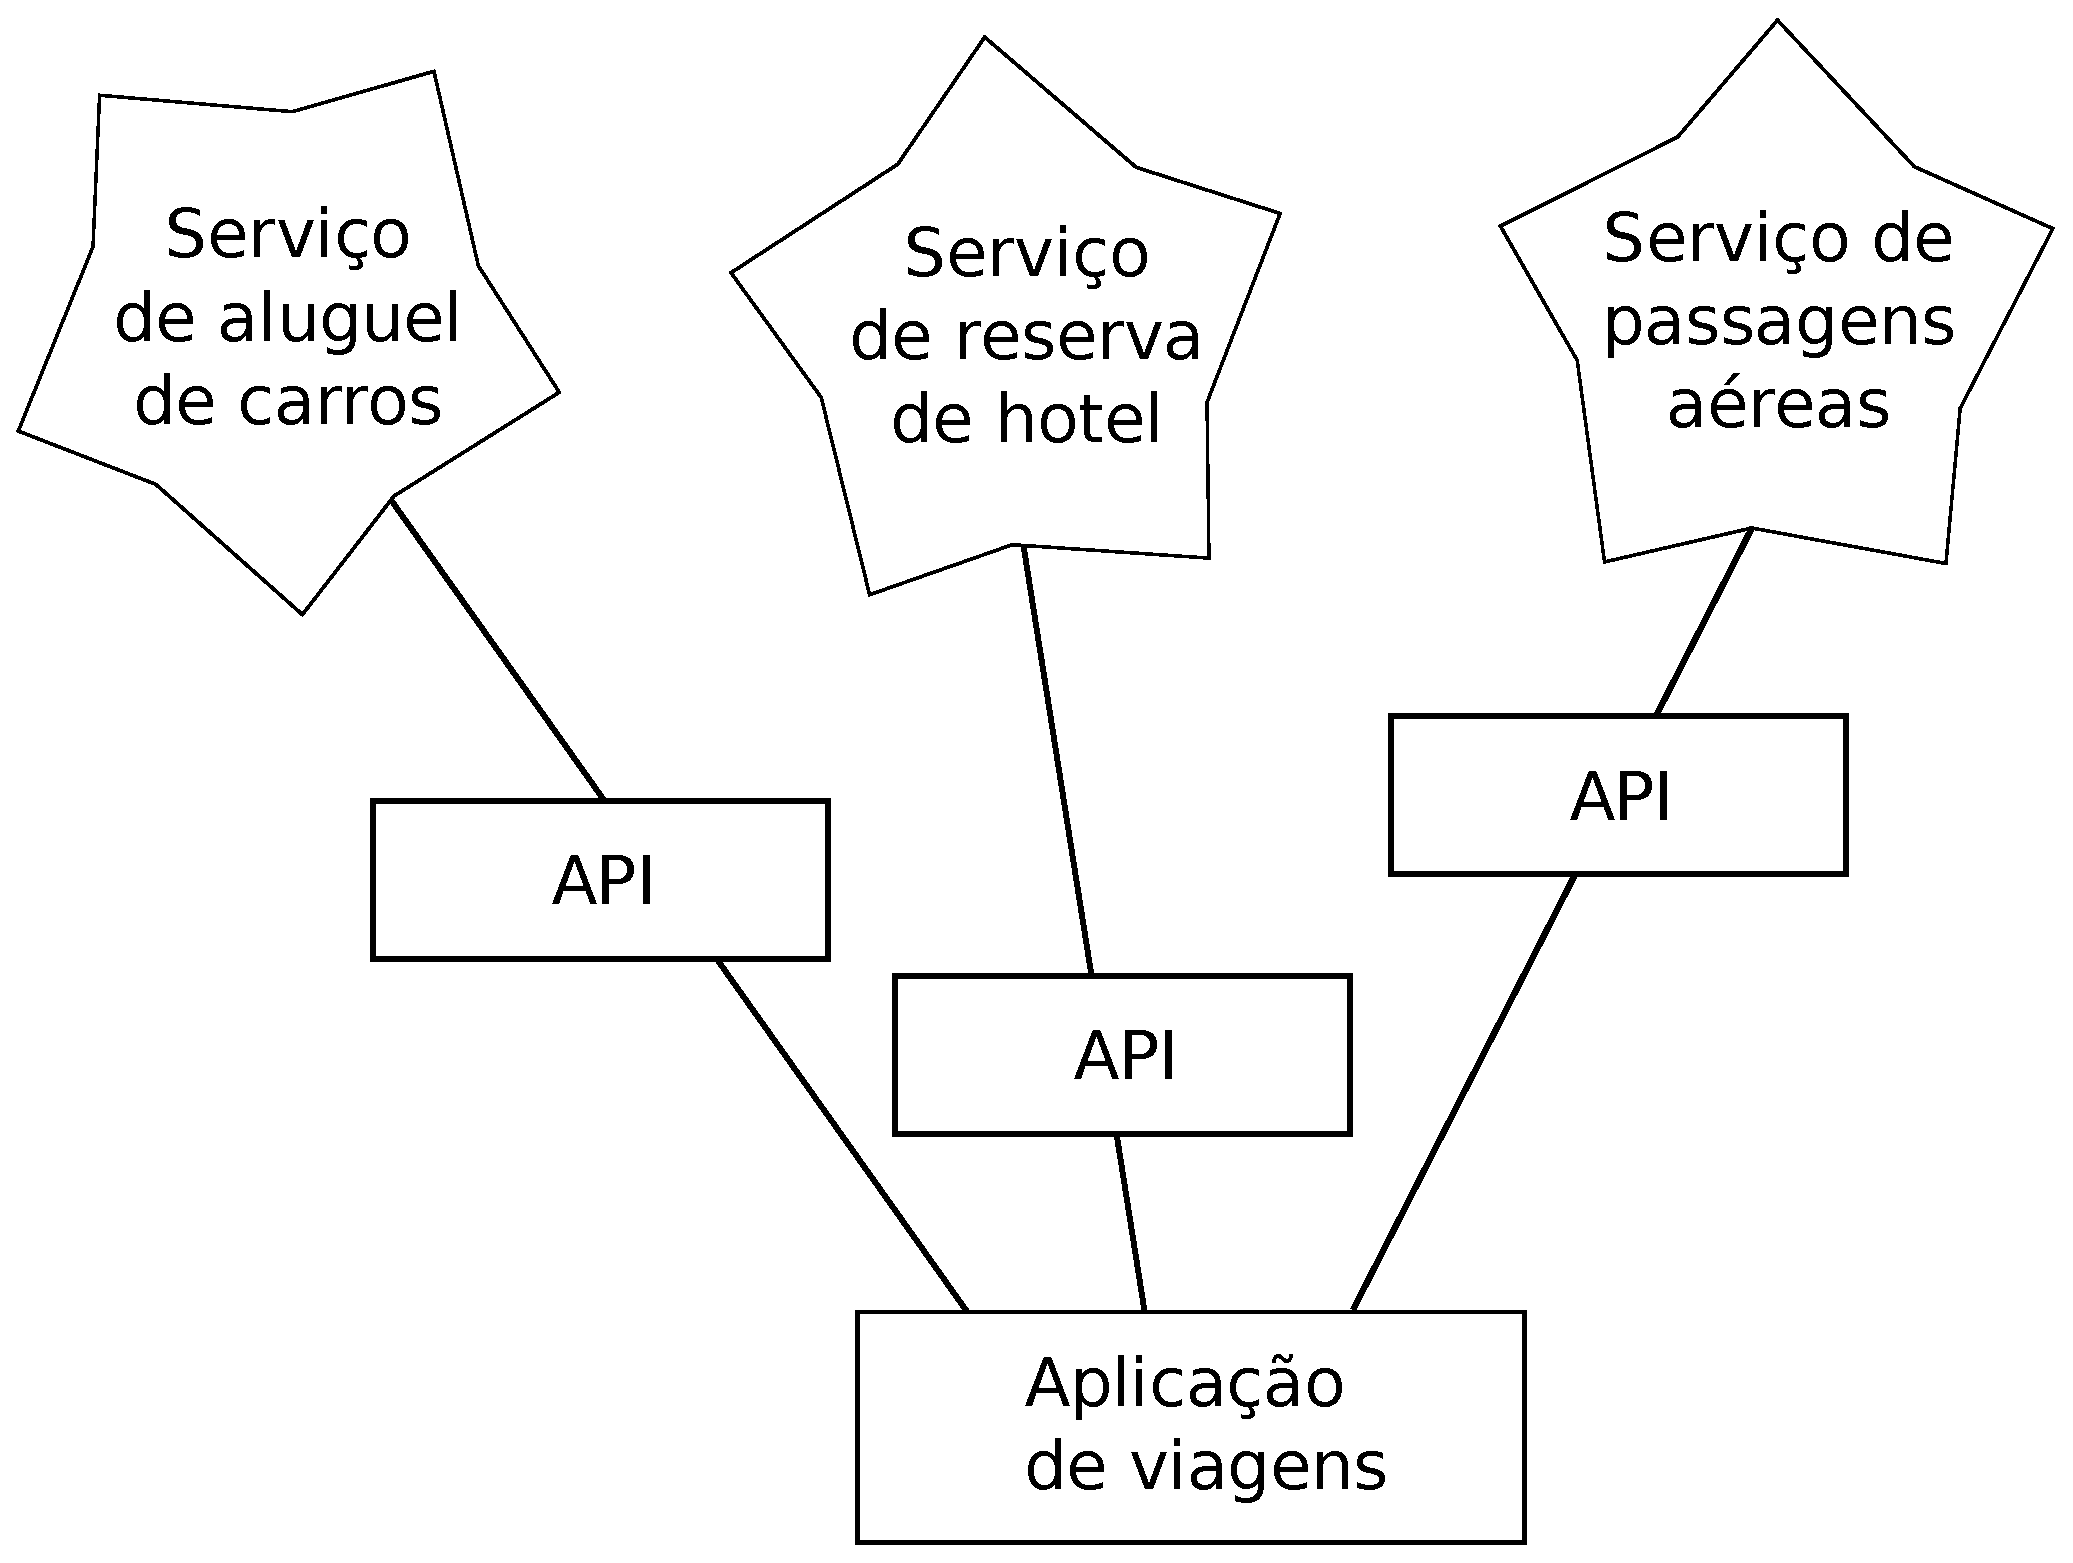
\includegraphics[height=2.50in]{figs2/soa.eps}}
\afterfig
Uma Arquitetura Orientada a Serviços tem muitas vantagens incluindo: (1)
nós sempre mantemos apenas uma cópia dos dados (isso é particularmente
importante para coisas como reservas de hotéis onde nós não queremos duplicá-las)
e (2) os donos dos dados podem criar regras sobre como usar os dados deles.
Com essas vantagens, um sistema SOA precisa ser cuidadosamente projetado
para ter boa performance e atender as necessidades dos usuários.
%A Service-Oriented Architecture has many advantages including: (1) we 
%always maintain only one copy of data (this is particularly important
%for things like hotel reservations where we do not want to over-commit)
%and (2) the owners of the data can set the rules about the use of their 
%data.   With these advantages, an SOA system must be carefully designed
%to have good performance and meet the user's needs.

Quando uma aplicação torna os serviços em sua API disponíveis para a internet,
nós os chamamos de {\bf serviços web}.
%When an application makes a set of services in its API available over the web, 
%we call these {\bf web services}. 

\section{Serviço Web Google de geocodificação}
%\section{Google geocoding web service}
\index{Google}
\index{geocodificação}
\index{serviço web}
%\index{Google}
%\index{geocoding}
%\index{web service}

O Google tem um excelente serviço web que nos permite usar seus bancos de
dados de informações geográficas. Nós podemos enviar uma pesquisa geográfica 
em forma de string como ``Ann Arbor, MI'' para a API de geodificação deles e o 
Google retornará o seu melhor palpite de em qual lugar do mapa nós podemos 
encontrar o local pesquisado e também nos falará sobre lugares nas proximidades. 
%Google has an excellent web service that allows us to make use of their 
%large database of geographic information.   We can submit a geographical
%search string like ``Ann Arbor, MI'' to their geocoding API and have Google 
%return its best guess as to where on a map we might find our search string and
%tell us about the landmarks nearby.

O serviço de geocodificação é grátis, porém limitado, então você não pode fazer
um uso ilimitado da API em serviços comerciais. Mas se você tem alguns dados de
localização que um usuário digitou em uma caixa de entrada, você pode usar
esta API para deixar suas informações mais concisas.
%The geocoding service is free but rate limited so you cannot make unlimited
%use of the API in a commercial application.   But if you have some survey data
%where an end user has entered a location in a free-format input box, you can use
%this API to clean up your data quite nicely.  

{\em Quando você está usando uma API grátis como a de geocodificação do Google,
você precisa ser respeitoso sobre o uso desses recursos. Se muitas pessoas
abusarem do serviço, o Google pode reduzir de forma significante seus serviços
gratuitos.}
\index{taxa de limitação}
%{\em When you are using a free API like Google's geocoding API, you need
%to be respectful in your use of these resources.  If too many people abuse the
%service, Google might drop or significantly curtail its free service.}
%\index{rate limiting}

Você pode ler documentos online sobre esse serviço, mas é bem simples e você
pode até testar ele usando um navegador, somente digitando a seguinte URL em
seu navegador:
%You can read the online documentation for this service, but it is quite simple
%and you can even test it using a browser by typing the following URL into your 
%browser:

\url{http://maps.googleapis.com/maps/api/geocode/json?sensor=false &address=Ann+Arbor%2C+MI}

Tenha certeza de resolver a URL e remover qualquer espaço em branco antes de 
colar a URL em seu navegador.
%Make sure to unwrap the URL and remove any spaces from the URL before pasting
%it into your browser.

A seguir temos uma simples aplicação que solicita ao usuário uma string de
pesquisa, requisita a API de geocodificação do Google, e extrai informações do
JSON que foi retornado.
%The following is a simple application to prompt the user for a search string,
%call the Google geocoding API, and extract information from the returned JSON.

\beforeverb
\begin{verbatim}
import urllib
import json

serviceurl = 'http://maps.googleapis.com/maps/api/geocode/json?'

while True:
    address = raw_input('Enter location: ')
    if len(address) < 1 : break

    url = serviceurl + urllib.urlencode({'sensor':'false', 
          'address': address})
    print 'Retrieving', url
    uh = urllib.urlopen(url)
    data = uh.read()
    print 'Retrieved',len(data),'characters'

    try: js = json.loads(str(data))
    except: js = None
    if 'status' not in js or js['status'] != 'OK':
        print '==== Failure To Retrieve ===='
        print data
        continue

    print json.dumps(js, indent=4)

    lat = js["results"][0]["geometry"]["location"]["lat"]
    lng = js["results"][0]["geometry"]["location"]["lng"]
    print 'lat',lat,'lng',lng
    location = js['results'][0]['formatted_address']
    print location
\end{verbatim}
\afterverb

O programa pega a string de pesquisa e constrói uma URL com a string
como um parâmetro devidamente codificado e então usa o {\bf urllib}
para retornar o texto da API de geodificação do Google. Diferente
de uma página web fixa, os dados que recebemos dependem dos parâmetros 
que nós enviamos e as informações geográficas armazenadas nos 
servidores do Google.
%The program takes the search string and constructs a URL with the
%search string as a properly encoded parameter and then uses
%{\bf urllib} to retrieve the text from the Google geocoding API.
%Unlike a fixed web page, the data we get depends on the parameters
%we send and the geographical data stored in Google's servers.

Uma vez que retornamos os dados JSON, nós os analisamos com a 
biblioteca {\bf json} e fazemos algumas checagens para garantir que 
recebemos a informação correta, então extraímos a informação de que 
necessitamos.
%Once we retrieve the JSON data, we parse it with the {\bf json}
%library and do a few checks to make sure that we received good data, 
%then extract the information that we are looking for.

A saída do programa está logo a seguir (algumas partes dos dados retornados
no JSON foram removidas):
%The output of the program is as follows (some of the returned
%JSON has been removed):

\beforeverb
\begin{verbatim}
$ python geojson.py
Enter location: Ann Arbor, MI
Retrieving http://maps.googleapis.com/maps/api/
  geocode/json?sensor=false&address=Ann+Arbor%2C+MI
Retrieved 1669 characters
{
    "status": "OK", 
    "results": [
        {
            "geometry": {
                "location_type": "APPROXIMATE", 
                "location": {
                    "lat": 42.2808256, 
                    "lng": -83.7430378
                }
            }, 
            "address_components": [
                {
                    "long_name": "Ann Arbor", 
                    "types": [
                        "locality", 
                        "political"
                    ], 
                    "short_name": "Ann Arbor"
                } 
            ], 
            "formatted_address": "Ann Arbor, MI, USA", 
            "types": [
                "locality", 
                "political"
            ]
        }
    ]
}
lat 42.2808256 lng -83.7430378
Ann Arbor, MI, USA
Enter location:
\end{verbatim}
\afterverb

Você pode baixar
\url{www.py4inf.com/code/geojson.py} e
\url{www.py4inf.com/code/geoxml.py} para explorar
variantes de JSON e XML da API de geocodificação do Google.
%You can download 
%\url{www.py4inf.com/code/geojson.py} and 
%\url{www.py4inf.com/code/geoxml.py} to explore the JSON
%and XML variants of the Google geocoding API. 

\section{Segurança e utilizanção de API}
\index{OAuth}
\index{API!chave}
%\section{Security and API usage}
%\index{OAuth}
%\index{API!key}

É bem comum que você necessite de algum tipo de 
``chave da API'' para fazer uso de uma API de um fornecedor.
A ideia geral é que eles querem saber quem está usando os
serviços deles e o quanto cada usuário está usando.
Entretanto elas têm partes pagas e gratuitas dos serviços
deles, ou uma política que limita o número de requisições
que um único indivíduo pode realizar durante um determinado
período de tempo.
%It is quite common that you need some kind of 
%``API key'' to make use of a vendor's API.  The
%general idea is that they want to know who is using 
%their services and how much each user is using.  
%Perhaps they have free and pay tiers of their services
%or have a policy that limits the number of requests 
%that a single individual can make during a particular 
%time period.

Uma vez que você tenha a chave da API, você simplesmente
insere a chave como parte dos dados do POST ou possivelmente
como um parâmetro da URL que está chamando a API.
%Sometimes once you get your API key, you simply include
%the key as part of POST data or perhaps as a parameter
%on the URL when calling the API.

Às vezes, o fornecedor quer aumentar a garantia da 
origem da requisição e então eles esperam que você os
envie mensagens criptografadas usando chaves compartilhadas
e secretas. Uma tecnologia muito comum que é utilizada para 
enviar requisições pela Internet é chamada {\bf OAuth}.
Você pode ler mais sobre o protocolo OAuth em 
\url{http://www.oauth.net}.
%Other times, the vendor wants increased assurance of
%the source of the requests and so they add expect you 
%to send cryptographically signed messages using shared
%keys and secrets.   A very common technology that is used 
%to sign requests over the Internet is called {\bf OAuth}.
%You can read more about the OAuth protocol at
%\url{http://www.oauth.net}.

Como a API do Twitter tornou-se cada vez mais valiosa, o
Twitter se transformou de uma API aberta e pública para uma API que
requisita o uso da assinatura OAuth em cada requisição.
Felizmente existe um bom número de bibliotecas OAuth 
convenientes e gratuitas então você pode evitar ter de escrever
uma implementação OAuth do início lendo sobre a especificação.
Estas bibliotecas são de complexidade variante e tem vários
graus de riqueza. O site do OAuth contém informações sobre
diversas bibliotecas OAuth.
%As the Twitter API became increasingly valuable, Twitter
%went from an open and public API to an API that required
%the use of OAuth signatures on each API request. Thankfully
%there are still a number of convenient and free OAuth libraries
%so you can avoid writing an OAuth implementation from scratch
%by reading the specification.  These libraries are of 
%varying complexity and have varying degrees of
%richness.  The OAuth web site has information about various 
%OAuth libraries.

Para o próximo exemplo nós vamos baixar os arquivos
{\bf twurl.py}, {\bf hidden.py}, {\bf oauth.py}, 
{\bf twitter1.py} a partir do 
\url{www.py4inf.com/code} e colocar todos na mesma pasta
no computador.
%For this next sample program we will download the files 
%{\bf twurl.py}, {\bf hidden.py}, 
%{\bf oauth.py}, 
%and
%{\bf twitter1.py} from 
%\url{www.py4inf.com/code} and put them all in a folder
%on your computer.

Para poder usar estes programas você vai precisar ter uma conta
no Twitter, e autorizar seu código Python como uma aplicação,
configurar uma key, secret, token e token secret. Você deverá 
editar o arquivo {\bf hidden.py} e armazenar
estas quatro strings nas variáveis apropriadas no arquivo:
%To make use of these programs you will need to have a Twitter
%account, and authorize your Python code as an application,
%set up a key, secret, token and token secret.  You will edit
%the file {\bf hidden.py} and put these four strings into the
%appropriate variables in the file:

\beforeverb
\begin{verbatim}
    def auth() :
        return { "consumer_key" : "h7L...GNg",
            "consumer_secret" : "dNK...7Q",
            "token_key" : "101...GI",
            "token_secret" : "H0yM...Bo" }
\end{verbatim}
\afterverb

O serviço web do Twitter é acessado utilizando uma URL como esta:
%The Twitter web service are accessed using a URL like this:

\url{https://api.twitter.com/1.1/statuses/user_timeline.json}

Uma vez que todas as informações de segurança tenham sido adicionadas,
a URL se parecerá com algo assim:
%But once all of the security information has been added, the URL
%will look more like:

\beforeverb
\begin{verbatim}
https://api.twitter.com/1.1/statuses/user_timeline.json?count=2
&oauth_version=1.0&oauth_token=101...SGI&screen_name=drchuck
&oauth_nonce=09239679&oauth_timestamp=1380395644
&oauth_signature=rLK...BoD&oauth_consumer_key=h7Lu...GNg
&oauth_signature_method=HMAC-SHA1
\end{verbatim}
\afterverb
%
Você pode ler a especificação OAuth, se você quiser saber mais
sobre o significado dos vários parâmetros que foram adicionados
para suprir os requerimentos de segurança do OAuth.
%You can read the OAuth specification if you want to
%know more about the meaning of the various parameters that
%are added to meet the security requirements of OAuth.  

Para os programas que nós executamos com o Twitter, nós escondemos toda
a complexidade nos arquivos {\bf oauth.py} e {\bf twurl.py}.
Nós simplesmente configuramos os segredos em {\bf hidden.py}
e então enviamos a URL desejada para a função 
{\bf twurl.augment()} e o código da biblioteca adiciona todos
os parâmetros necessários à URL para nós.
%For the programs we run with Twitter, we hide all the 
%complexity in the files {\bf oauth.py} and {\bf twurl.py}.
%We simply set the secrets in {\bf hidden.py} and then 
%send the desired URL to the {\bf twurl.augment()} 
%function and the library code adds all the necessary 
%parameters to the URL for us.

Este programa ({\bf twitter1.py}) recupera a linha de tempo
de um usuário do Twitter em particular e retorna isso para nós
no formato JSON em uma string. Então nós simplesmente exibimos
os primeiros 250 caracteres da string:
%This program ({\bf twitter1.py}) retrieves the timeline
%for a particular Twitter user and returns it to us in JSON
%format in a string.  We simply print the first 250 characters
%of the string:

\beforeverb
\begin{verbatim}
import urllib
import twurl

TWITTER_URL='https://api.twitter.com/1.1/statuses/user_timeline.json'

while True:
    print ''
    acct = raw_input('Enter Twitter Account:')
    if ( len(acct) < 1 ) : break
    url = twurl.augment(TWITTER_URL,
        {'screen_name': acct, 'count': '2'} )
    print 'Retrieving', url
    connection = urllib.urlopen(url)
    data = connection.read()
    print data[:250]
    headers = connection.info().dict
    # print headers
    print 'Remaining', headers['x-rate-limit-remaining']
\end{verbatim}
\afterverb

Quando o programa é executado, ele produz a seguinte saída:
%When the program runs it produces the following output: 
 
\beforeverb
\begin{verbatim}
Enter Twitter Account:drchuck
Retrieving https://api.twitter.com/1.1/ ...
[{"created_at":"Sat Sep 28 17:30:25 +0000 2013","
id":384007200990982144,"id_str":"384007200990982144",
"text":"RT @fixpert: See how the Dutch handle traffic 
intersections: http:\/\/t.co\/tIiVWtEhj4\n#brilliant",
"source":"web","truncated":false,"in_rep
Remaining 178

Enter Twitter Account:fixpert
Retrieving https://api.twitter.com/1.1/ ...
[{"created_at":"Sat Sep 28 18:03:56 +0000 2013",
"id":384015634108919808,"id_str":"384015634108919808",
"text":"3 months after my freak bocce ball accident, 
my wedding ring fits again! :)\n\nhttps:\/\/t.co\/2XmHPx7kgX",
"source":"web","truncated":false,
Remaining 177

Enter Twitter Account:
\end{verbatim}
\afterverb

Juntamente com a linha de tempo retornada, o Twitter também 
retorna metadados sobre a requisição no header da resposta HTTP.
Uma header em particular, {\bf x-rate-limit-remaining}, nos 
informa quantas requisições ainda podemos realizar antes que sejamos
bloqueados por um curto período de tempo. Você pode ver que nossas
requisições restantes irão diminuir em um a cada vez que fazemos 
uma requisição a esta API.
%Along with the returned timeline data, Twitter also returns
%metadata about the request in the HTTP response headers. 
%One header in particular, {\bf x-rate-limit-remaining}, informs
%us how many more requests we can make before we will be shut 
%off for a short time period.  You can see that our remaining 
%retrievals drop by one each time we make a request to the 
%API.

No exemplo a seguir, nós requisitamos os amigos de um usuário do
Twitter, analisamos o JSON retornado, e extraímos algumas informações
sobre os amigos. Nós também descartamos o JSON depois de analisar e
fazer uma ``impressão bonita'' dele com uma indentação de quatro
caracteres para nos permitir estudar os dados quando nós quisermos
extrair mais campos.
%In the following example, we retrieve a user's Twitter friends,
%parse the returned JSON, and extract some of the information
%about the friends.  We also dump the JSON after parsing and
%``pretty-print'' it with an indent of four characters to allow
%us to pore through the data when we want to extract more fields.

\beforeverb
\begin{verbatim}
import urllib
import twurl
import json

TWITTER_URL = 'https://api.twitter.com/1.1/friends/list.json'

while True:
    print ''
    acct = raw_input('Enter Twitter Account:')
    if ( len(acct) < 1 ) : break
    url = twurl.augment(TWITTER_URL,
        {'screen_name': acct, 'count': '5'} )
    print 'Retrieving', url
    connection = urllib.urlopen(url)
    data = connection.read()
    headers = connection.info().dict
    print 'Remaining', headers['x-rate-limit-remaining']
    js = json.loads(data)
    print json.dumps(js, indent=4)

    for u in js['users'] :
        print u['screen_name']
        s = u['status']['text']
        print '  ',s[:50]
\end{verbatim}
\afterverb

Desde que o JSON se tornou próximo das listas e dicionários do Python,
nós pudemos usar uma combinação de operações pelo index e o laço
{\tt for} para vasculhar os dados retornados com muito pouco 
código em Python.
%Since the JSON becomes a set of nested Python lists and dictionaries,
%we can use a combination of the index operation and {\tt for} loops to 
%wander through the returned data structures with very little 
%Python code.

A saída do programa se parece como a seguir (alguns itens dos dados
estão encurtados para caberem na página):
%The output of the program looks as follows (some of the data items 
%are shortened to fit on the page):

\beforeverb
\begin{verbatim}
Enter Twitter Account:drchuck
Retrieving https://api.twitter.com/1.1/friends ...
Remaining 14
{
    "next_cursor": 1444171224491980205, 
    "users": [
        {
            "id": 662433, 
            "followers_count": 28725, 
            "status": {
                "text": "@jazzychad I just bought one .__.", 
                "created_at": "Fri Sep 20 08:36:34 +0000 2013", 
                "retweeted": false, 
            }, 
            "location": "San Francisco, California", 
            "screen_name": "leahculver", 
            "name": "Leah Culver", 
        }, 
        {
            "id": 40426722, 
            "followers_count": 2635, 
            "status": {
                "text": "RT @WSJ: Big employers like Google ...", 
                "created_at": "Sat Sep 28 19:36:37 +0000 2013", 
            }, 
            "location": "Victoria Canada", 
            "screen_name": "_valeriei", 
            "name": "Valerie Irvine", 
    ], 
    "next_cursor_str": "1444171224491980205"
}
leahculver
   @jazzychad I just bought one .__.
_valeriei
   RT @WSJ: Big employers like Google, AT&amp;T are h
ericbollens
   RT @lukew: sneak peek: my LONG take on the good &a
halherzog
   Learning Objects is 10. We had a cake with the LO,
scweeker
   @DeviceLabDC love it! Now where so I get that "etc

Enter Twitter Account:
\end{verbatim}
\afterverb

A última parte da saída é onde vemos o laço for lendo os
cinco ``amigos'' recentes da conta do Twitter {\bf drchuck} e
imprimindo os status mais recentes de cada amigo. Tem muito mais dados
disponíveis para se utilizar no JSON retornado. Se você olhar na 
saída do programa, você pode ver também que a ``procura de amigos'' de
uma conta em particular tem diferentes níveis de limitação que 
o número de consultas de linha do tempo que podemos executar por 
período de tempo.
%The last bit of the output is where we see the for loop reading the
%five most recent ``friends'' of the {\bf drchuck} Twitter account 
%and printing the most recent status for each friend. There is a 
%great deal more data available in the returned JSON.  If you look
%in the output of the program, you can also see that the ``find the friends''
%of a particular account has a different rate limitation than 
%the number of timeline queries we are allowed to run per time period.

Estas chaves seguras da API permitem ao Twitter ter uma sólida confiança
que eles sabem quem está utilizando a API, quais dados e em que níveis. A
técnica da taxa limite de utilização nos permite fazer simples, consultas de 
dados pessoais, mas não nos permite desenvolver um produto que pega dados
da API milhões de vezes por dia.
%These secure API keys allow Twitter to have solid confidence that they 
%know who is using their API and data and at what level.   The 
%rate-limiting approach allows us to do simple, personal data retrievals but
%does not allow us to build a product that pulls data from their API 
%millions of times per day.

\section{Glossário}
%\section{Glossary}

\begin{description}

\item[API:] Interface de Programação de Aplicação - Um contrato entre
aplicações que define os padrões de interação entre dois componentes
de aplicação.
\index{API}
%\item[API:] Application Program Interface - A contract between
%applications that defines the patterns of interaction between 
%two application components.
%\index{API}

\item[ElementTree:] Uma biblioteca feita em Pyhon que é utilizada para
analisar dados XML.
\index[ElementTree]
%\item[ElementTree:] A built-in Python library used to parse XML data.
%\index{ElementTree}

\item[JSON:] JavaScript Object Notation. Um formato que permite a
marcação de dados estruturados baseados na sintaxe de objetos do
JavaScript.
\index{JSON}
\index{JavaScript Object Notation}
%\item[JSON:] JavaScript Object Notation. A format that allows for 
%the markup of structured data based on the syntax of JavaScript
%Objects.
%\index{JSON}
%\index{JavaScript Object Notation}

\item[SOA:]  Arquitetura Orientada a Serviços. Quando uma aplicação
é feita de componentes conectados através da internet.
\index{SOA}
zindex{Arquitetura Orientada a Serviços}
%\item[SOA:] Service-Oriented Architecture. When an application is 
%made of components connected across a network.
%\index{SOA}
%\index{Service Oriented Architecture}

\item[XML:] eXtensible Markup Language. Um formato que permite a
marcação de dados estruturados.
\index{XML}
\index{eXtensible Markup Language}
%\item[XML:] eXtensible Markup Language. A format that allows for 
%the markup of structured data.
%\index{XML}
%\index{eXtensible Markup Language}

\end{description}

\section{Exercícios}
%\section{Exercises}

\begin{ex}
Altere o
\url{www.py4inf.com/code/geojson.py} ou
\url{www.py4inf.com/code/geoxml.py} para exibir os
dois caracteres do código do país dos dados retornados.
Adicione um verificador de erros, para que seu programa
não procure se o código do país não estiver lá. Uma vez
que você tenha isso funcionando, procure por 
``Oceano Atlantico'' e tenha certeza que o código consegue
lidar com localizações que não estão em nenhum país.
\end{ex}
%Change either the 
%\url{www.py4inf.com/code/geojson.py} or
%\url{www.py4inf.com/code/geoxml.py} to print out the 
%two-character country code from the retrieved data.
%Add error checking so your program does not traceback
%if the country code is not there.  Once you have it 
%working, search for ``Atlantic Ocean'' and make sure
%it can handle locations that are not in any country.
%\end{ex}

